\documentclass[11pt]{article}

\usepackage[margin=1.1in]{geometry}
\usepackage[T1]{fontenc}
\usepackage{microtype}
\usepackage{amsmath,amssymb,amsthm}
\usepackage{booktabs}
\usepackage{graphicx}
\usepackage{array}
\usepackage{longtable}
\usepackage{xurl}
\usepackage{needspace}
\usepackage[numbers,sort&compress]{natbib}
\usepackage[hidelinks]{hyperref}
\hypersetup{
  pdftitle={Trace Sampling at the Collector Boundary: Costs and Diagnostic Evidence},
  pdfauthor={Victor Bona},
  pdfsubject={Distributed tracing; sampling; diagnostic evidence; observability},
  pdfkeywords={distributed tracing, head sampling, tail sampling, observability, OpenTelemetry, measurement study}
}
\newtheorem{theorem}{Theorem}[section]
\newtheorem{lemma}[theorem]{Lemma}
\newtheorem{corollary}[theorem]{Corollary}
\newtheorem{proposition}[theorem]{Proposition}
\theoremstyle{definition}
\newtheorem{definition}[theorem]{Definition}
\newtheorem{remark}[theorem]{Remark}
\newcommand{\artifact}[1]{\nolinkurl{#1}}
\makeatletter
\newcommand{\tableinput}[1]{\@@input #1 }
\makeatother
\emergencystretch=1em

\title{Trace Sampling at the Collector Boundary:\\Costs and Diagnostic Evidence}
\author{Victor Bona\\[2pt]
\small Independent Researcher, Blumenau, Brazil\\
\small \texttt{victor.bona@hotmail.com}}
\date{September 2026}

\newcommand{\MainCells}{70}
\newcommand{\MainTraces}{1,400,000}
\newcommand{\MainSpans}{7,042,000}
\newcommand{\FullCPU}{0.77}
\newcommand{\FullRSS}{184.1}
\newcommand{\IngressMin}{9.950}
\newcommand{\IngressMax}{9.958}
\newcommand{\MaxLagMS}{3.69}
\newcommand{\TailTenCPUIncrease}{47.9}
\newcommand{\HeadTenIngress}{89.9}
\newcommand{\HeadTenJSON}{89.9}
\newcommand{\HeadTenCPU}{77.0}
\newcommand{\HeadTenCPULo}{74.4}
\newcommand{\HeadTenCPUHi}{79.6}
\newcommand{\HeadTenGzip}{89.8}
\newcommand{\HeadTenRSS}{174.0}
\newcommand{\TailTenIngress}{0.0}
\newcommand{\TailTenJSON}{89.2}
\newcommand{\TailTenCPU}{-47.9}
\newcommand{\TailTenCPULo}{-52.6}
\newcommand{\TailTenCPUHi}{-43.1}
\newcommand{\TailTenGzip}{89.0}
\newcommand{\TailTenRSS}{233.5}

\newcommand{\LiveCells}{60}
\newcommand{\LiveRequests}{180,000}
\newcommand{\LiveFaults}{5,400}
\newcommand{\LiveHeadAccuracy}{10.1}
\newcommand{\LiveTailAccuracy}{69.4}
\newcommand{\CalibrationRejects}{0}
\newcommand{\HoeffdingRadius}{89.8}
\newcommand{\CommonHeadSemanticCorrect}{52}
\newcommand{\CommonTailSemanticCorrect}{45}
\newcommand{\CommonSemanticCases}{600}
\newcommand{\LiveMaxLagMS}{21.02}

\newcommand{\CostCells}{96}
\newcommand{\CostBlocks}{8}
\newcommand{\CostTailRetained}{290}
\newcommand{\CostMaxLagMs}{3.34}

\newcommand{\TaskFullCorrect}{568}
\newcommand{\TaskFullAccuracy}{94.67}
\newcommand{\TaskAlpha}{0.283}
\newcommand{\TaskHeadAccuracy}{92.10}
\newcommand{\TaskHeadBound}{4.53}
\newcommand{\TaskHeadDiscard}{20}
\newcommand{\TaskTailAccuracy}{92.02}
\newcommand{\TaskTailBound}{4.60}
\newcommand{\TaskTailDiscard}{20}
\newcommand{\LoadCells}{80}
\newcommand{\LoadFullCore}{40.0}
\newcommand{\LoadFullCPU}{14.00}
\newcommand{\LoadHeadCore}{7.1}
\newcommand{\LoadHeadCPU}{2.50}
\newcommand{\LoadHeadSaving}{82.2}
\newcommand{\LoadTailCore}{63.7}
\newcommand{\LoadTailCPU}{22.28}
\newcommand{\LoadTailSaving}{-59.1}
\newcommand{\LoadAllTailCore}{76.1}
\newcommand{\LoadAllTailCPU}{26.62}
\newcommand{\LoadAllTailSaving}{-90.1}

\newcommand{\SensitivityThreshold}{45.31}
\newcommand{\WindowTwentyFull}{92.50}
\newcommand{\WindowTwentyHeadDiscard}{20}
\newcommand{\WindowTwentyHeadAccuracy}{90.14}
\newcommand{\WindowTwentyHeadBound}{4.86}
\newcommand{\WindowTwentyTailDiscard}{20}
\newcommand{\WindowTwentyTailAccuracy}{90.22}
\newcommand{\WindowTwentyTailBound}{4.90}
\newcommand{\WindowFiftyFull}{98.83}
\newcommand{\WindowFiftyHeadDiscard}{35}
\newcommand{\WindowFiftyHeadAccuracy}{96.50}
\newcommand{\WindowFiftyHeadBound}{3.41}
\newcommand{\WindowFiftyTailDiscard}{35}
\newcommand{\WindowFiftyTailAccuracy}{96.46}
\newcommand{\WindowFiftyTailBound}{3.46}
\newcommand{\WindowTwoHundredFull}{100.00}
\newcommand{\WindowTwoHundredHeadDiscard}{80}
\newcommand{\WindowTwoHundredHeadAccuracy}{97.72}
\newcommand{\WindowTwoHundredHeadBound}{3.01}
\newcommand{\WindowTwoHundredTailDiscard}{65}
\newcommand{\WindowTwoHundredTailAccuracy}{99.06}
\newcommand{\WindowTwoHundredTailBound}{1.44}
\newcommand{\BoundaryGateSaving}{82.3}
\newcommand{\BoundaryCollectorSaving}{-2.9}
\newcommand{\BoundaryTailSaving}{-58.3}

\newcommand{\WindowHeadMCSE}{0.21}
\newcommand{\WindowTailMCSE}{0.37}
\newcommand{\WindowNetLossMCSE}{0.40}

\newcommand{\PlacementFileGateSaving}{80.5}
\newcommand{\PlacementFileUniformSaving}{-3.2}
\newcommand{\PlacementFileTailSaving}{-53.9}
\newcommand{\PlacementDualGateSaving}{83.4}
\newcommand{\PlacementDualUniformSaving}{24.2}
\newcommand{\PlacementDualTailSaving}{-13.9}
\newcommand{\PlacementFileUniformIncrease}{3.2}
\newcommand{\HighBatchRate}{5,000}
\newcommand{\HighBatchShortDifference}{+2.02}
\newcommand{\HighBatchShortInterval}{[+1.90, +2.15]}
\newcommand{\HighBatchLongDifference}{+2.02}
\newcommand{\HighBatchLongInterval}{[+1.92, +2.13]}

\begin{document}
\maketitle
\begin{abstract}
Trace retention is an incomplete predictor of observability cost: a sampler changes where work is avoided, how spans are grouped for export, and which evidence remains available. We study these effects in OpenTelemetry Collector Contrib v0.136.0 on one shared node with loopback transport. Five randomized blocks cross sampler placement with export path at 40,000 offered spans/s. Native uniform sampling at nominal 10\% retention increases Collector CPU by \PlacementFileUniformIncrease{}\% with JSON-only export and reduces it by \PlacementDualUniformSaving{}\% with JSON plus Jaeger. A pre-ingress gate retains identical trace IDs but avoids ingestion and excludes selection work from the Collector endpoint. Retain-all controls show that stateful release changes batching and CPU without discarding traces. A short-timeout CPU reduction at 250 spans/s disappears at 5,000 spans/s, where tail increases CPU at both tested timeouts. A separate SDK comparison, load sweep, and delivery probes distinguish application work, Collector resources, and complete evidence delivery. An illustrative localization task uses measured HTTP timings and ideal offline sampling without an SDK or Collector. Its results show how window size and selection-dependent reference evidence affect a fixed median-change scorer, conditional on the observed corpus. The study supports evaluating sampling at explicit component boundaries, measuring batching and serialization alongside trace counts, and defining the diagnostic evidence objective before selecting a rate. The research archive preserves frozen protocols, raw observations, failed attempts, and executable checks.

\end{abstract}
\noindent\textbf{Keywords:} distributed tracing; head sampling; tail sampling; diagnostic evidence; OpenTelemetry; reproducible evaluation.

\section{Introduction}\label{sec:introduction}
Trace sampling is often configured as a percentage, yet that percentage does not identify the work avoided by an observability pipeline. A decision before Collector ingress can avoid receiving and decoding discarded spans. The same decision after ingress preserves those costs and introduces processor work. A stateful tail sampler also changes when traces are released, affecting batches and export framing. Consequently, two configurations that retain the same traces can have different costs, and even retaining every trace can change CPU consumption.

Distributed tracing systems have long balanced information retention against overhead~\cite{sigelman2010dapper,kaldor2017canopy}. Contemporary samplers additionally optimize diagnostic utility using structural diversity, runtime state, or analysis results~\cite{lascasas2019sifter,huang2024trastrainer,zhu2025unisage}. These objectives make it necessary to separate three measurements: retained trace count, resource consumption at a specified component, and evidence available to a specified diagnostic task.

This paper studies that separation through matched controls in OpenTelemetry. The principal comparisons vary identical uniform selections before and inside the Collector, export path, batch timeout, and offered load. Retain-all tail controls reveal costs that retained span counts cannot explain. A controlled localization example then illustrates how evidence-window size and selection policy affect a specified diagnostic task.

We address four questions:
\begin{enumerate}
\item \textbf{RQ1:} How does sampler placement change Collector cost when uniform policies retain identical trace IDs?
\item \textbf{RQ2:} How do batching and exporter configuration affect Collector cost at equal span retention?
\item \textbf{RQ3:} How do offered load and sampling policy affect Collector CPU, memory, and exported volume?
\item \textbf{RQ4:} In a controlled localization example, how do window size and selection policy affect available evidence and accuracy?
\end{enumerate}

The contribution is an empirical account of these interactions for a pinned Collector and explicitly measured configurations. Matching trace IDs controls selection content in RQ1; replaying identical input controls the workload in RQ2; randomized runtime blocks characterize repeatability. The localization example supplies a transparent task whose evidence requirements can be inspected. The scope is a component-level measurement study of established policies, with elementary probability results supplying its reference model.

\section{Background and related work}\label{sec:related}
\paragraph{Collection architecture and cost.}
A trace links causally related spans through a propagated context~\cite{W3CTraceContext}. Head sampling can avoid recording and exporting spans when performed in the software development kit (SDK); a gate after span construction can avoid only subsequent work~\cite{OTelSamplingSpec,otelSampling}. Our pre-ingress gate measures the Collector boundary. Centralized tail processing receives spans from the full offered stream. Retroactive architectures such as Hindsight instead retrieve selected data from local buffers~\cite{Hindsight2023}, so the ingestion cost of our treatment is architecture-specific. Mint separates shared trace patterns from variable parameters at agents, retaining a compact representation of all requests and fuller information for selected ones~\cite{huang2024mint}. Its compressed representation and our whole-trace retention endpoint measure different forms of data reduction.

\paragraph{Sampling for diagnostic utility.}
Sifter favors traces poorly represented by its learned model~\cite{lascasas2019sifter}. Sieve combines structural and latency encoding with an adapted robust random cut forest~\cite{huang2021sieve}. TraStrainer uses runtime-state preferences and diversity~\cite{huang2024trastrainer}; TracePicker evaluates anomaly and trace-pattern preservation~\cite{xie2025tracepicker}. UniSage analyzes correlated telemetry before selecting traces and logs~\cite{zhu2025unisage}. Gleaner combines event-pair sets, including log information, with alarm-guided quotas and diversity selection~\cite{yang2026gleaner}. These systems establish diagnostic utility as a sampling objective. Our matched policies expose collection and export effects that a comparison of retention fractions alone leaves unresolved; the study does not rank these alternative algorithms.

\paragraph{Diagnostic evidence and delivery.}
Spectroscope compares request flows across normal and problem periods~\cite{sambasivan2011spectroscope}. MicroRank and TraceRCA use richer localization procedures involving reference behavior and service relationships~\cite{yu2021microrank,li2021tracerca}. Our three-candidate median-change task is an illustrative model of reference-dependent evidence, rather than an implementation of either localizer.

Complete delivery is a separate prerequisite. The pinned tail processor makes decisions after a wait measured from the first received span; its default is 30\,s. Buffers, decision caches, and late arrivals can change what is actually exported~\cite{otelTailSampling0136}. Our supporting delivery probes use a deliberately shorter two-second wait and controlled arrival order. They demonstrate these documented mechanisms, while the principal resource experiments use complete-trace arrivals. Span completion and arrival order must be distinguished: OpenTelemetry permits children to remain active after a parent ends~\cite{otelSpanLifecycle}.

\paragraph{Measurement and uncertainty.}
Tracing-overhead measurement requires attention to recorded content and measurement boundaries~\cite{reichelt2026tracingoverhead}. Coehlo et al. examine uncertainty in sampled trace aggregates~\cite{coehlo2012uncertainty}; unequal-probability weighting can estimate totals but cannot recover a discarded evidence item~\cite{HorvitzThompson1952}. We use paired runtime comparisons for resource effects~\cite{nistPairedObservations} and Monte Carlo standard errors to describe randomized-replay precision conditional on the fixed localization corpus.


\section{Model and diagnostic criterion}\label{sec:model}
Fix a population of $N\ge1$ traces. Ideal uniform sampling retains each complete trace independently with probability $p\in[0,1]$. An ideal protected-tail policy retains every trace satisfying a fixed predicate and independently retains other traces with probability $r\in[0,1]$. Let $\alpha$ be the protected fraction and $b$ the expected retained trace fraction. These models describe selection; native hash decisions and stateful delivery are measured separately.

Diagnostic value requires an endpoint. A stipulated witness set $W_j$ contains $m_j\ge1$ traces, each sufficient for a defined evidence predicate. Its one-witness endpoint is $D_j(S)=\mathbf1\{S\cap W_j\ne\varnothing\}$ for retained set $S$. In the localization example, a fixed scorer instead compares reference and incident windows. Let $B_i\in\{0,1\}$ be full-data correctness for incident $i$, and $A_{i,a}\in\{0,1\}$ correctness under sampling configuration $a$, counting abstention as incorrect. For a uniform draw $I$ from the fixed corpus and fresh sampling randomness, the expected accuracy loss is
\begin{equation}\label{eq:loss-target}
 \Delta_a=\mathbb E[B_I]-\mathbb E[A_{I,a}].
\end{equation}
This example evaluates retention of evidence for a known task. Its corpus, incident windows, candidate services, and scorer are fixed.

\section{Formal results}\label{sec:theory}
Under independent complete-trace selection, at least one of $m\ge1$ interchangeable witnesses survives with probability $1-(1-p)^m$, whereas retaining all $d\ge1$ required traces has probability $p^d$. For any fixed $p<1$, the latter approaches zero as the number of required traces grows. Thus a retention rate alone cannot guarantee a task-independent minimum success probability. A window of $w$ requests supplies $wp$ retained requests in expectation, so window size also determines the amount of available evidence. Neither identity determines a scorer's accuracy.

For the protected-tail policy, linearity of expectation gives, for $0\le\alpha<1$ and $b\in[\alpha,1]$,
\begin{equation}\label{eq:tailbudget}
 b=\alpha+(1-\alpha)r,\qquad r=\frac{b-\alpha}{1-\alpha}.
\end{equation}
When $\alpha>0$ and $b<1$, $r<b$: protection reduces unprotected inclusion at equal expected trace budget. Budgets below $\alpha$ are infeasible if every protected trace must survive. Equal trace budgets need not imply equal byte budgets. Appendix~\ref{app:mathematical-supplement} provides proofs, witness thresholds, and the full window-count identities.

\section{Resource accounting and estimation}\label{sec:cost}
For additive trace sizes $v_i$ and inclusion probabilities $\pi_i$, linearity gives $\mathbb E[V_{\rm out}]=\sum_i\pi_i v_i$. Export envelopes, compression, and sampler-added metadata require additional accounting. We measure Collector CPU, sampled peak resident set size (RSS), accepted spans, and serialized output separately.

A linear reference model separates fixed work $F$, work before selection $U$, downstream work $D$, and additional sampling work $A_H,A_T$, all nonnegative:
\begin{align}
 C_1&=F+U+D,& C_H&=F+A_H+p(U+D),\nonumber\\
 C_T&=F+U+A_T+b_VD,&&\label{eq:cost-model}
\end{align}
where $b_V$ is the retained downstream byte fraction. Sampling overhead includes only work inside the chosen measurement boundary; the pre-ingress gate's own CPU is outside our Collector endpoint. Here the head gate precedes $U$, whereas the tail processor follows it. Consequently,
\begin{equation}\label{eq:savings}
 C_1-C_H=(1-p)(U+D)-A_H,\qquad
 C_1-C_T=(1-b_V)D-A_T.
\end{equation}
An in-Collector uniform sampler has the same placement-dependent form as $C_T$, with its own sampling overhead and retained byte fraction. Sampling after ingress can save CPU when avoided downstream work exceeds added work; the sign requires measurement.

These equations assume a fixed downstream cost per retained byte and unchanged grouping. Stateful release can violate that approximation: batch count, resource/scope grouping, encoding, and export fanout can change even with full span retention. The retain-all tail intervention tests this distinction directly. The model explains possible signs but its coefficients are not identified from total CPU.

Tail state also creates a capacity requirement. Under finite-mean stationary conditions and the arrival regularity required by Little's theorem, mean buffered occupancy is $\lambda W$ for admitted arrival rate $\lambda$ and mean residence time $W$~\cite{Little1961}. Mean occupancy is not a bound on bursts. Our finite measurements characterize the configured Collector boundary, including export work, rather than long-run saturation or monetary savings.

\section{Experimental method}\label{sec:methods}
\subsection{Design and environment}
Table~\ref{tab:design} identifies the experiments and their units. Each has a protocol and source freeze before measured execution, fixed seeds, randomized execution order, and archived functional pilots excluded from estimates. Resource experiments repeat runtime measurements; the localization example varies evidence on a fixed observed corpus.

All workloads execute in isolated namespaces of a single-node Kubernetes testbed on one shared AMD Ryzen 7 5825U node: eight cores, sixteen logical CPUs, approximately 30.8\,GiB allocatable memory, Linux 6.6.68, and k3s v1.30.4+k3s1. Collector Contrib v0.136.0 and Python 3.12.10 are pinned. Resource transports use loopback; Collector and Jaeger use GOMAXPROCS=2. Placement and higher-load batching use six-CPU/10-GiB runner limits. The low-load exporter runner has four CPUs and 4\,GiB; load and localization runners have four CPUs and 6\,GiB. Contrasts pair treatments within campaigns; different campaigns are not pooled.

\begin{table}[htbp]
\centering\small
\begin{tabular}{>{\raggedright\arraybackslash}p{.25\linewidth}>{\raggedright\arraybackslash}p{.27\linewidth}>{\raggedright\arraybackslash}p{.38\linewidth}}
\toprule
Experiment & Measured units & Purpose \\
\midrule
Sampler placement & 40 cells, five blocks & Matched selections crossed with export path \\
Exporter/batching & 96 cells, eight blocks & Fixed input at 250 offered spans/s \\
Batching at higher load & 20 cells, five blocks & Retain-all versus bypass at 5,000 spans/s \\
Load sweep & 80 cells, five blocks & Resource effects at 250--100,000 offered spans/s \\
Live SDK comparison & 60 cells, five blocks & Application and Collector resource costs \\
Localization example & 600 observed incidents & Nested windows and selection-dependent evidence \\
\bottomrule
\end{tabular}
\caption{Runtime blocks and observed incidents are distinct units. The localization example has 5,000 conditional replay trials per configuration across forty-eight configurations. Supporting delivery probes are specified in Section~\ref{sec:delivery-results}.}
\label{tab:design}
\end{table}

\subsection{Matched sampler placement}\label{sec:boundary-method}
Five randomized blocks cross full retention, a pre-ingress uniform gate, an in-Collector probabilistic sampler before batching, and nominal 10\% tail with JSON-only or JSON-plus-Jaeger export. Each cell offers 8,000 complete five-span traces/s before selection. Every hundred traces contain one ERROR and one 400\,ms root; other roots last 10\,ms. SHA-256-derived trace IDs and phase/sequence attributes identify the synthetic input, grouped in requests of at most one hundred traces.

The uniform treatments retain exactly the same IDs using the pinned probabilistic processor's \texttt{hash\_seed} mode, seed 1729, and configured 10\%~\cite{otelProbabilistic0136}. A separate FNV-1a32 implementation reconstructs selection from fourteen-bit buckets below 1638, corresponding to a uniform-bucket fraction of 9.9976\%. The in-Collector treatment receives the complete input and adds native sampling tracestate. The placement contrast therefore includes selection and metadata work as well as the avoided ingress.

Tail protects ERROR or trace duration at least 250\,ms, and otherwise uses native probabilistic selection with background $0.08/0.98$. It has a two-second decision wait, 161,000 trace slots, and 1,288,000 entries per decision cache. Common batch settings are timeout 1,000\,ms, target 1,024 spans, and maximum 2,048. Each cell starts fresh processes and storage, warms up for five seconds, drains for five, measures thirty seconds of load, and drains for five more. Preparation, startup, trace queries, shutdown, and archival compression are outside the CPU endpoint.

Excluded capacity pilots test 100,000, 40,000, then 10,000 offered spans/s, stopping at the highest rate that meets delivery, scheduling, and throttling criteria. At 100,000, Jaeger's successful-save count remains incomplete at the final scrape; 40,000 passes. Collector export acknowledgments alone are insufficient because the pinned Jaeger receiver queues backend work~\cite{jaegerSpanProcessor176}. Both warmup and final save counters must match all selected spans supplied to date, with zero save errors. The final CPU snapshot follows the counter scrape. CPU direction is not a rate-selection criterion.

\subsection{Fixed-input exporter and batching intervention}\label{sec:export-method}
A single archived checkout/steady corpus supplies 500 warmup and 3,000 measured requests with five spans each. It was recorded from an OpenTelemetry Python 1.37.0 application executing HTTP and PostgreSQL operations. Trace IDs, parent links, statuses, attributes, and durations are preserved; one common timestamp translation moves the corpus into the backend query window. Input payload bytes are identical across treatments. Replay offers ten complete traces every 200\,ms, or 250 spans/s.

Eight randomized blocks cross JSON-only versus JSON-plus-Jaeger export, batch timeout 100 versus 1,000\,ms, and bypass versus retain-all tail versus nominal 10\% tail. Batch target 256/maximum 512, tail decision wait two seconds, capacity 512, and both decision caches 10,000 remain fixed. Both tail modes evaluate ERROR, latency, and background policies in the same order without first-match short circuiting. Retain-all tail sets the background probability to one; the sampled mode uses $0.08/0.98$.

The additional exporter sends compressed OpenTelemetry Protocol (OTLP) HTTP protobuf to Jaeger 1.76.0 with local Badger storage~\cite{jaegerDeployment176,jaegerCli176,otelOtlpHttp0136}. The Collector exporter's queue and retries are disabled. Collector, Jaeger, and the store start fresh per cell; Jaeger also runs without receiving traces in JSON-only cells. Ten seconds of warmup and five of drain precede the sixty-second measured schedule and common five-second final drain. A twelve-cell setup pilot is excluded. Primary contrasts compare each tail mode with bypass within exporter/timeout combinations; every paired block is retained.

The higher-load experiment crosses bypass and retain-all tail with the same two timeouts and dual export in five blocks. It cyclically replays the same SDK templates with distinct trace IDs and translated timestamps, preserving span content and appending phase/sequence/template identifiers. Requests still contain ten traces, now offered at 5,000 spans/s. All treatments within a block receive identical bytes. Tail slots/caches match the placement experiment; batch target/maximum remain 256/512. Warmup, measurement, and drain durations match the low-load experiment. The 256-span target is close to one second of the original 250-span/s stream, exposing timeout effects; the higher-load study retains that target, while placement retains the sweep's 1,024/2,048 settings for comparability. Cloned templates increase offered load, not the number of independently observed application requests.

An initial five-second capacity pilot accepted 20,000 spans/s, but the first measured cell failed the final backend-save equality check, and execution stopped. A recorded amendment required full sixty-second pilots at the next predefined candidates: 10,000 failed the 0.5\,s scheduling-lag limit; 5,000 passed all four treatments. That rate was frozen before the twenty-cell campaign. This operating point is limited by the harness's pacing criterion, not an identified Collector capacity: the 10,000-span/s pilot completed delivery but missed generator scheduling, using ten-trace requests rather than placement's hundred-trace requests. The failed measured attempt and excluded pilots remain archived; none contributes to the paired estimates. Acceptance criteria and measurement windows were unchanged.

\subsection{Offered-load sweep}\label{sec:load-method}
The sweep uses the same synthetic five-span construction as the placement experiment at 50, 2,000, 8,000, and 20,000 traces/s. Five randomized blocks cross every rate with full retention, a pre-ingress BLAKE2b gate at 10\%, nominal 10\% tail, and retain-all tail. Tail capacity, caches, batching, and measurement durations match the placement experiment. The sweep's gate has a different hash from the matched placement controls, so its aggregate results are reported separately.

An excluded setup pilot selected the upper rate by a predefined criterion: at least 0.25 mean Collector cores, scheduling lag below 0.5\,s, and complete delivery. The eighty measured cells use fixed settings at all rates. Selection, span content, and counters must reconcile without early drop, refusal, or failed export. Shutdown must add no output beyond the endpoint. CPU ticks, RSS samples, schedule lag, and throttling are archived for every cell.

\paragraph{Separate SDK resource measurements.}
A retained live study crosses checkout and document applications, steady and bursty arrivals averaging fifty requests/s, and full retention, SDK head, and tail policies in five randomized blocks, sixty cells in total. Python OpenTelemetry 1.37.0 applies parent-based trace-ID-ratio head selection at 10\%~\cite{otelPythonSampler137}. Each cell has ten seconds of warmup, sixty seconds of requests, and five seconds of final drain, using real HTTP and PostgreSQL operations, Collector export to Jaeger, and a JSON mirror. SQL errors, delayed queries, and domain-invariant faults each affect 1\% of measured requests. Application CPU sums gateway and worker process time. Its paired resource contrasts provide a separate boundary comparison.

\subsection{Illustrative localization task}\label{sec:diagnosis-method}
The example tests how retained reference evidence affects a specified scorer. A gateway visits three loopback HTTP leaf handlers in one Python process, with no nested leaf calls. Background delays are lognormal with median 8\,ms and log standard deviation 0.5. The driver constructs four-span OTLP-format traces from actual server timestamps and the enclosing request interval. All statuses are OK; cause labels and injection controls are absent from observed attributes. Sampling is ideal offline replay, without an SDK or Collector.

The 600 incidents cross three affected services, added delays 5/15\,ms, affected-request probabilities 0.5/1, and fifty seeds per combination. Incident order is randomized, with at most eight workers. Each incident has 200 reference and 200 incident requests; nested prefixes of 20, 50, and 200 form paired views of the same incidents. The scorer predicts the candidate service with the largest retained median increase,
\begin{equation}\label{eq:scorer}
 h_s=\operatorname{median}(d_{s,\rm incident})-
     \operatorname{median}(d_{s,\rm reference}).
\end{equation}
Even-count medians average the middle values; service-name order breaks ties. A nonpositive maximum still produces a prediction. Either empty window causes abstention, counted as incorrect. Both windows are sampled. All full-data errors remain. Candidate services and incident boundaries are supplied, so this is a closed-set localization task; a uniform random guess among the balanced candidates has accuracy one third.

A disjoint 2,000-request healthy calibration fixes the nearest-rank 95th percentile of root duration before collecting incidents. Tail protects roots at or above this threshold. For each window size, the measured corpus-wide protected fraction determines $r$ through Equation~\eqref{eq:tailbudget}, equalizing expected trace budgets. The expected fractions are 5\%, 10\%, 20\%, 35\%, 50\%, 65\%, 80\%, and 95\%; infeasible tail budgets remain recorded. A separate twelve-incident functional pilot is excluded without tuning accuracy.

There are 5,000 randomized replay trials per configuration. Trial $t$ uses Python \texttt{Random} with seed $1990000+t$ to draw an incident uniformly with replacement and 400 trace priorities shared across all windows, budgets, and policies. This implements the declared ideal iid replay model. Trials estimate a fixed-corpus average; they are not additional observed incidents.

\subsection{Measurement, inference, and validation}\label{sec:validation-method}
Collector CPU is user-plus-system process time over measured load and drain, from endpoint snapshots with 0.01\,s tick resolution. RSS is sampled approximately once per second in the low-load exporter experiment and every 500\,ms in the other replay experiments. JSON is uncompressed serialized output; accepted-span counts exclude transport framing. Placement and higher-load batching additionally report Jaeger CPU and their process sum. Generator CPU covers sending and monitoring during the window; input construction and pre-ingress selection occur in excluded preparation and are not timed. Complete JSON outputs are reconstructed independently. In these two experiments, backend save counters cover every selected span, while post-endpoint trace queries check sixteen selected traces per phase and dual-export cell. This is a content sample, not a durability test. Study cells execute sequentially, and archive transfers follow measured collection.

For a resource contrast, the runtime block is the replication unit. Pointwise intervals are $\bar x\pm t_{0.975,n-1}s/\sqrt n$, with five or eight paired differences. The study reports every configured primary contrast and all blocks, without significance-based selection.

For the localization example, we report sampled accuracy and paired net loss $\overline Z_a$, where $Z_{t,a}=B_{I_t}-A_{I_t,a}\in\{-1,0,1\}$ includes improvements as negative losses. Monte Carlo standard errors are $s/\sqrt{5000}$ using the sample standard deviation of correctness or paired loss. They measure precision over randomized replay conditional on the fixed corpus. Complete configuration results remain in the artifact.

\paragraph{AI-assisted research workflow.}
OpenAI Codex assisted protocol design, literature discovery, the workload and orchestration programs, analysis and validation code, mathematical derivations and proof code, and figure-generation code. Automated workloads collected the measurements in the Kubernetes testbed. Timings and resource counters are archived program observations. Codex also assisted manuscript drafting and revision. The validation implementations are part of the same AI-assisted research workflow, not external replication. Source freezes, raw observations, and executable checks make these steps inspectable. The author retains responsibility for the methods, claims, source attribution, and final text.

\section{Results}\label{sec:results}
\subsection{RQ1: placement and export path at matched retention}\label{sec:placement-results}
Table~\ref{tab:boundary} crosses placement with export path at 40,000 offered spans/s. Native uniform sampling increases Collector CPU by \PlacementFileUniformIncrease{}\% with JSON-only export, but reduces it by \PlacementDualUniformSaving{}\% with JSON plus Jaeger. Each direction occurs in every paired block. The export-path interaction, defined as the dual-export minus JSON-only difference in native-minus-full CPU, is $-2.162$ CPU-seconds, with pointwise 95\% interval $[-2.390,-1.934]$.

\begin{table}[htbp]
\centering\small
\setlength{\tabcolsep}{3.5pt}
\begin{tabular}{lrlrrr}
\toprule
Policy & Collector & CPU saving versus full & Jaeger & JSON & RSS \\
& CPU (s) & \% [95\% interval] & CPU (s) & \% & MiB \\
\midrule
\tableinput{fifth-placement-rows.tex}
\bottomrule
\end{tabular}
\caption{Placement crossed with export path, five randomized blocks. CPU spans thirty seconds of offered load plus five seconds of drain and final counter scrapes. Savings average paired block percentages; JSON is relative to the matching full-retention mean. RSS is the mean per-cell sampled Collector peak. The pre-ingress gate admits only selected spans; all other paths receive the full input. Uniform selections match exactly. Negative savings mean increased CPU. Intervals are pointwise.}
\label{tab:boundary}
\end{table}

In the reference model of Equation~\eqref{eq:savings}, the JSON result corresponds to sampler work exceeding avoided downstream work; adding OTLP export reverses that balance for native uniform sampling. The same intervention reduces the tail penalty from 53.9\% to 13.9\%, but tail still increases Collector CPU. The boundary matters even within one configuration: with dual export, Collector-plus-Jaeger process CPU falls from 51.72\,s under full retention to 10.09\,s under native uniform and 13.10\,s under tail.

The pre-ingress gate saves \PlacementFileGateSaving{}\% and \PlacementDualGateSaving{}\% of Collector CPU in the respective export paths. It is the favorable Collector-only reference in which discarded input never reaches that process and selection work is excluded. Native uniform receives the complete input, selects the same IDs, and adds 44 serialized bytes of tracestate per retained span. Its JSON output is 11.4\% of full, compared with 10.1\% for the gate. Equal selections therefore do not make either the work or serialized representation equal.

All forty cells meet the delivery and pacing criteria. Maximum scheduling lag is 309.7\,ms, with no throttling, refusal, failed export, or early tail eviction.

\subsection{RQ2: batching costs at equal span retention}\label{sec:batch-results}
Bypass and retain-all tail export every span in each fixed-input cell. At 250 offered spans/s with JSON plus Jaeger, retain-all tail reduces Collector CPU relative to bypass at the 100\,ms batch timeout and increases it at 1,000\,ms. The respective mean differences are $-0.173$ and $+0.066$ CPU-seconds over sixty seconds plus five seconds of drain. Both directions occur in all eight paired blocks. Bypass consumes 0.249--0.603 CPU-seconds across the original configurations, below 1\% of one core.

\begin{figure}[htbp]
\centering
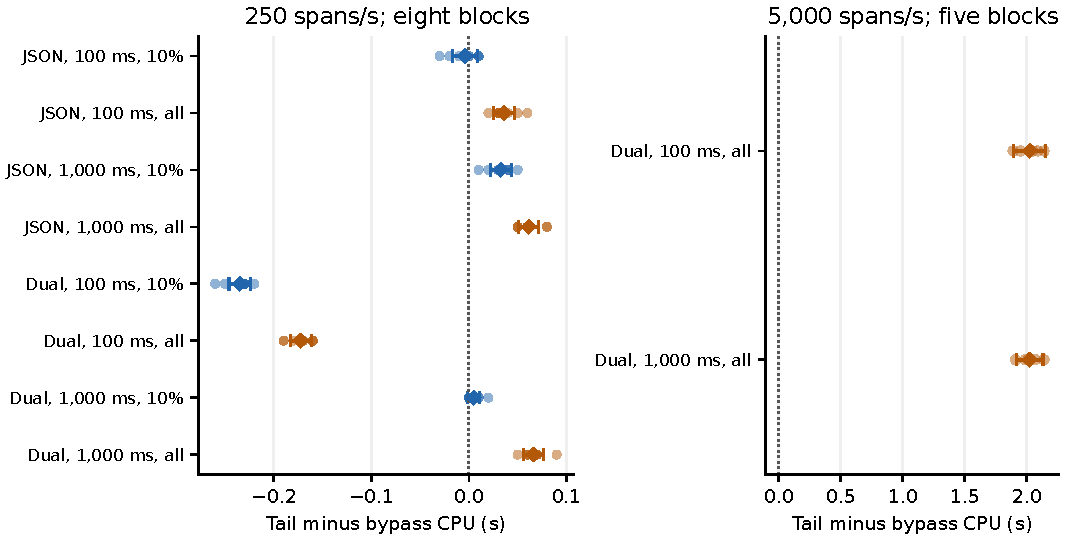
\includegraphics[width=\linewidth]{figures/controlled-cost-contrasts.pdf}
\caption{Fixed-input Collector CPU contrasts with bypass. Dots are paired runtime-block differences; diamonds and bars show means and pointwise 95\% Student-$t$ intervals. The original 250-span/s study has eight blocks; the separate 5,000-span/s study has five. Both measure sixty seconds of load plus five seconds of drain. The panels use different horizontal scales. Negative values mean less CPU than bypass. ``Dual'' means JSON plus Jaeger; ``all'' denotes retain-all tail.}
\label{fig:controlled-cost}
\end{figure}

At the lower rate, bypass sends 300 batches of fifty spans with the short timeout and sixty batches of 250 with the long timeout. Retain-all tail sends approximately sixty batches with either setting. The pinned processor's one-second policy ticker and per-trace forwarding explain how stateful release changes grouping~\cite{otelTailProcessor0136}. Adding Jaeger changes the retain-all tail-minus-bypass contrast by $-0.209$\,s at the short timeout but only $+0.005$\,s at the long timeout.

The reversal does not persist at the new 5,000-span/s operating point. Retain-all tail increases Collector CPU at both timeouts in every paired block. Mean differences are \HighBatchShortDifference{}\,s at 100\,ms, with interval \HighBatchShortInterval{}, and \HighBatchLongDifference{}\,s at 1,000\,ms, with interval \HighBatchLongInterval{}. Bypass now consumes about 4.9 CPU-seconds, or 7.6\% of one core over the measured window. Its 1,000 batches are all size-triggered at both timeouts. Tail emits 1,200 and 1,154 batches at the short and long timeouts respectively. It therefore no longer reduces batch count relative to bypass. Figure~\ref{fig:controlled-cost} reports both higher-rate contrasts alongside the original ones.

The batch target is a trigger rather than an exact output size~\cite{otelBatchProcessor0136}. Bypass adds fifty spans per request and crosses the 256-span target at 300; tail forwards five-span traces individually and crosses it at 260. At 100\,ms, residuals flush between policy releases: each measured cell records 1,139 size-triggered 260-span batches and 61 partial timeout batches. At 1,000\,ms, residuals accumulate across releases, giving 1,153 batches of 260 spans and one final timeout batch of 220, or $\lceil300{,}000/260\rceil=1{,}154$. These counts reconstruct all 300,000 measured spans in every block.

Serialization changes at equal span retention too. In the original measured corpus, bypass emits 600 resource/scope groups while retain-all tail emits 6,000, increasing JSON from about 4.99 to 7.05 million bytes. The file exporter serializes the grouping it receives~\cite{otelFile0136}. Reducing batch count can therefore coexist with increased serialized volume. Trace count, grouping, bytes, and CPU describe different properties of the pipeline.

\subsection{RQ3: resource effects across offered load}\label{sec:load-results}
Figure~\ref{fig:load-sweep} reports all four offered rates and policies. At the upper rate, full retention consumes \LoadFullCPU{} Collector CPU-seconds, or \LoadFullCore{}\% of one core over the nominal 35-second window. Nominal 10\% tail uses \LoadTailCPU{}\,s, a paired increase of 59.1\%, while exported JSON falls to 10.9\% of full. Retain-all tail uses still more CPU despite identical retained span counts. Tail memory rises with offered load, consistent with the cost of retaining undecided trace state.

\begin{figure}[htbp]
\centering
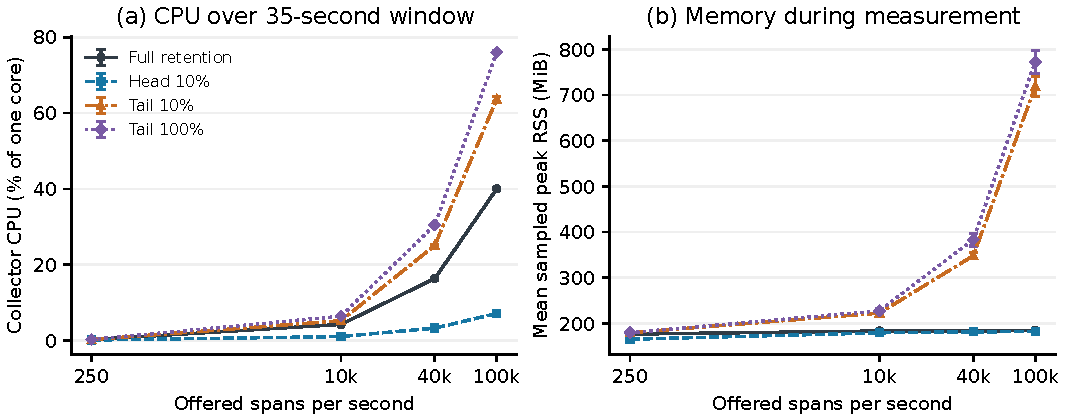
\includegraphics[width=\linewidth]{figures/load-sweep.pdf}
\caption{Collector load sweep with JSON file export, five runtime blocks per point. Error bars are pointwise 95\% Student-$t$ intervals. CPU refers to one core over the nominal 35-second window. Memory is mean per-cell sampled peak RSS. Capacity and batch settings are common across treatments. ``Head 10\%'' denotes the pre-ingress BLAKE2b gate; it is a different selection implementation from the matched controls in Table~\ref{tab:boundary}.}
\label{fig:load-sweep}
\end{figure}

At the upper rate, the pre-ingress gate saves \LoadHeadSaving{}\% of Collector CPU. Table~\ref{tab:load-high} reports all upper-rate treatments. The separate matched-placement experiment in RQ1, at 40,000 spans/s, demonstrates why a pre-ingress saving does not describe native probabilistic processing of full input; it is not a same-rate control for this 100,000-span/s point. For the tail path, avoided export work is insufficient to offset additional work at the upper JSON-only boundary. The fixed-input results in RQ2 establish that this sign is configuration-dependent.


\begin{table}[htbp]
\centering\small
\begin{tabular}{lrlrr}
\toprule
Policy & CPU (s) & CPU saving (\%, 95\% interval) & JSON (\%) & RSS (MiB) \\
\midrule
\tableinput{load-high-rows.tex}
\bottomrule
\end{tabular}
\caption{The separate load sweep at 100,000 offered spans/s, five paired blocks. CPU spans thirty seconds of offered load plus five seconds of drain. JSON is relative to full retention; RSS is the mean sampled per-cell peak. Negative savings mean greater cost. Head denotes the pre-ingress BLAKE2b gate.}
\label{tab:load-high}
\end{table}

All eighty cells reconcile complete selected traces, with no throttling, refusal, failed export, or early tail drop. These finite windows establish an observed operating point rather than a saturation limit.

\paragraph{SDK placement at a separate application boundary.}
The retained live application study supplies the SDK comparison. At fifty requests/s, SDK head sampling reduces combined gateway/worker process CPU by 15.4--18.0\% and Collector CPU by 31.3--36.5\% across its four application/traffic conditions (Table~\ref{tab:sdk-resources}). Those measurements include application execution and instrumentation, so their magnitudes differ from the pre-ingress gate's Collector-only savings. This separate experiment does not hold input or exporter configuration constant against the load sweep.

\begin{table}[htbp]
\centering\small
\begin{tabular}{lll}
\toprule
Application/traffic & Application CPU saving (\%) & Collector CPU saving (\%) \\
\midrule
\tableinput{sdk-resource-rows.tex}
\bottomrule
\end{tabular}
\caption{SDK head sampling at nominal 10\%, relative to full retention in the separate live study. Values are mean paired savings with pointwise 95\% intervals over five blocks. S denotes steady traffic and B bursty traffic. Application CPU sums the gateway and worker processes.}
\label{tab:sdk-resources}
\end{table}

\subsection{RQ4: an illustrative evidence-window dependence}\label{sec:task-results}
Table~\ref{tab:window-cohort} reports the full-data baselines and calibrated protection across the paired window sizes. Increasing window size improves full-data accuracy before sampling is applied. The healthy-root threshold is \SensitivityThreshold{}\,ms; in the incident mixture it protects about 13\% of traces, making the two smallest tail budgets infeasible. Protection is more frequent in incident windows than in reference windows.

\begin{table}[htbp]
\centering\small
\begin{tabular}{rrrrr}
\toprule
Requests per & Full-data & Full-data & \multicolumn{2}{c}{Protected traces (\%)} \\
window & correct/total & accuracy (\%) & Reference & Incident \\
\midrule
\tableinput{window-cohort-rows.tex}
\bottomrule
\end{tabular}
\caption{The same 600 incidents at three nested window sizes. Protected means root duration at least the calibrated healthy 95th percentile. Each size has its own full-data baseline. All errors remain; the window configurations are dependent.}
\label{tab:window-cohort}
\end{table}

Figure~\ref{fig:window-evidence} connects accuracy to the evidence remaining in each window. At 20\% expected retention with 200 requests per window, head correctly localizes 97.72\% of replay cases and tail 92.68\%, with Monte Carlo standard errors \WindowHeadMCSE{} and \WindowTailMCSE{} percentage points respectively. Head retains about forty requests in each window. Tail retains means of 25.3 reference and 54.2 incident requests. The calibrated rule changes both the allocation of comparison evidence and the retained duration distributions. Prioritizing slow requests can therefore work against this reference-dependent scorer.

\begin{figure}[htbp]
\centering
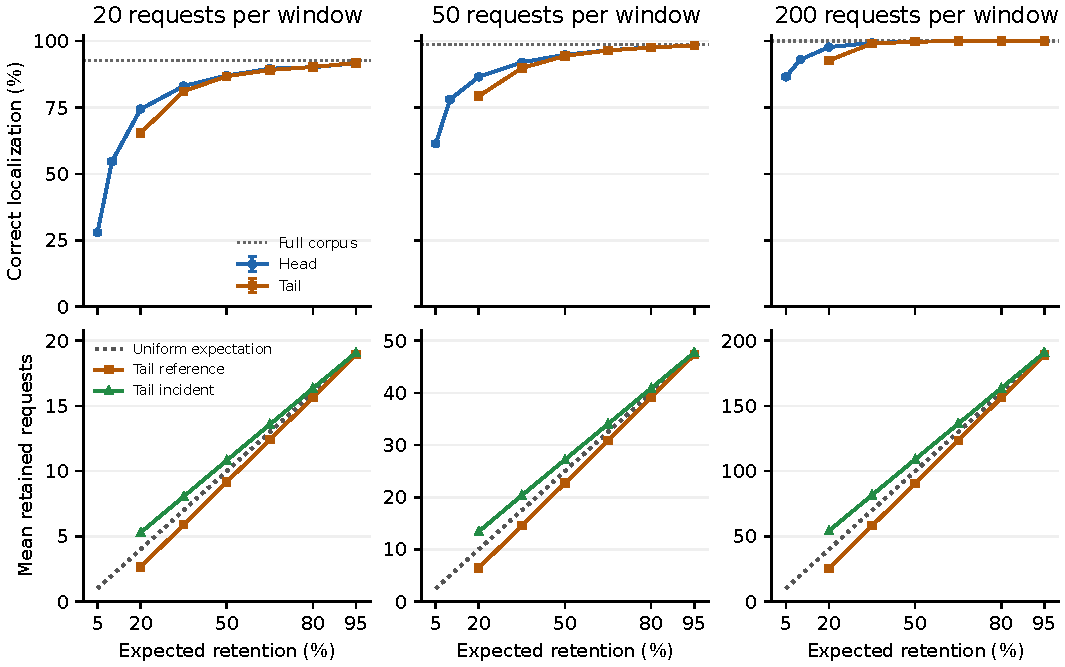
\includegraphics[width=\linewidth]{figures/window-evidence.pdf}
\caption{Illustrative localization on the fixed corpus. Upper panels show replay accuracy with one Monte Carlo standard error, often smaller than the marker; exact full-corpus baselines are dotted. Lower panels show mean retained reference and incident requests under tail; the uniform reference line is the analytical expectation $wp$ for either window. Tail has no feasible points at 5\% or 10\% retention. Lines connect tested rates and do not establish accuracy at intermediate rates.}
\label{fig:window-evidence}
\end{figure}

The dependence concerns both the scorer's baseline and its evidence after selection. At the twenty-request size and 65\% head retention, 260 harmful changes and 139 gains give observed net loss of 2.42 percentage points, with Monte Carlo standard error \WindowNetLossMCSE{} points. The paired calculation includes both outcomes. Increasing replay trials can reduce this simulation uncertainty, but adds no observed incidents. Complete configurations, losses, gains, abstentions, retained counts, and descriptive strata remain in the artifact.

\Needspace{10\baselineskip}
\subsection{Supporting delivery checks}\label{sec:delivery-results}
These probes connect documented tail-processor behavior to an explicit complete-witness predicate. A matched $2^4$ design crosses an early received root ERROR marker, an immediate or five-second-delayed decisive database leaf, decision caches enabled or disabled, and churn/capacity. Each combination repeats with three seeds and 200 seven-span failed traces. The decision wait is two seconds. Churn inserts 300 normal traces into 256 slots; its control has no churn and 50,000 slots. The churn factor therefore changes load and capacity jointly. Timing pairs share input content within other factors.

\begin{table}[htbp]
\centering\small
\begin{tabular}{llllrrr}
\toprule
Root ERROR & Leaf & Cache & Churn & IDs & Spans & Complete \\
\midrule
\tableinput{matched-probe-summary-rows.tex}
\bottomrule
\end{tabular}
\caption{Matched protected-only probes, per cell with 200 failed traces. Rows group equivalent factor outcomes; every reported result repeats in all three seeds. Complete witnesses require the stipulated span identities, parent links, and decisive leaf evidence. ``Either'' denotes both tested levels.}
\label{tab:matched}
\end{table}

An early received root ERROR preserves all complete witnesses in the tested combinations. Without that marker, immediate delivery preserves all witnesses while delayed delivery preserves none. With churn and no decision cache, delayed ERROR leaves can be exported without their discarded ancestors. A nonsampled cache can instead preserve the drop decision and export none. A separate burst probe with sixteen trace slots retains sixteen of 200 failures and records 184 early drops. The pinned processor documentation describes these decision, cache, and eviction mechanisms~\cite{otelTailSampling0136}.

Full configurations, additional probes, and partial-span interventions are retained in the artifact. Section~\ref{sec:discussion} states the delivery and evidence-predicate limitations.


\section{Discussion and threats to validity}\label{sec:discussion}
\subsection{Implications for operators}
Begin a sampling comparison by locating the decision and the measured cost. A gate before Collector ingress, an SDK decision, and a Collector processor avoid different work. Report accepted spans, exported bytes, Collector CPU, and sampled memory separately. Match retained IDs when comparing placement, and inspect metadata additions: equal trace selections need not yield equal serialized volume.

Treat batch formation as part of the sampling configuration. Measure exporter fanout and actual batch counts alongside timeout settings. A retain-all control is useful because it exposes buffering and grouping effects without discarding evidence. Its cost relative to bypass includes those effects, so it should not be interpreted as pure decision overhead. The results also show why a resource sign measured with JSON export should be rechecked for the deployed exporter path.

Define the diagnostic evidence before choosing a retention rate. Report protected and unprotected classes separately. For tasks using reference windows, record the number and distribution of retained reference observations as well as incident observations. Evaluate the actual scorer's full-data accuracy and an explicit deterioration margin at representative window sizes. Mean retention alone does not establish either quantity.

Finally, validate delivery independently of ideal selection. Measure decisive-span arrival relative to the first received span and decision time; test trace affinity, cache outcomes, and buffer capacity under bursts. The supporting probes in Section~\ref{sec:delivery-results} show that exported ERROR leaves can coexist with missing ancestors. Size memory for measured residence times and bursts, then verify under load.

\subsection{Construct and statistical validity}
The placement experiment controls retained trace IDs but changes ingestion, processor work, and sampling metadata together. Tail comparisons additionally change selection content and stateful processing. The fixed-input experiment controls span content while varying exporter fanout and batch timeout; actual grouping is observed. Higher-load replay also scales state capacity and adds identification attributes, so cross-campaign comparisons do not isolate load alone. Batch-size targets are fixed within campaigns, not crossed as a sensitivity factor; the RQ1 sign is established at target 1,024, not for all batch targets. These designs estimate configured treatment contrasts rather than universal per-span costs.

Resource intervals describe five or eight randomized runtime blocks on a shared node. They are pointwise, and small sample sizes do not establish the Student-$t$ assumptions. Process ticks, finite drains, and sampled RSS limit precision; sampled peaks can miss shorter transients. Replaying a fixed corpus characterizes runtime repeatability rather than independent application workloads.

The localization example is intentionally small: three HTTP handlers in one process, constructed lognormal delays, known incident boundaries, and a supplied candidate set. It measures a fixed median-change task, not unknown-incident detection or human debugging. Healthy reference windows are not no-fault incident controls. Window size changes both the full-data baseline and evidence redundancy. Calibrating on separate healthy requests prevents fault-outcome tuning of the threshold, but using the corpus-wide protected mass to equalize expected budgets remains an offline condition. A deployment must estimate that mass under changing traffic.

The 5,000 replay trials quantify uncertainty over randomized selections and incident draws from one fixed corpus under the declared iid model. They add no observed incidents. Shared priorities and nested windows create dependence between comparisons. The reported standard errors quantify conditional Monte Carlo precision and do not establish performance for particular services or strata. Inference over an incident population would require a sampling design and assumptions beyond this conditional example.

\subsection{External validity and reproducibility}
The measured resource effects apply to one shared node, loopback transport, a pinned historical Collector release, GOMAXPROCS=2, and the specified JSON or JSON-plus-Jaeger paths. JSON file export supplies an inspectable endpoint; it is not representative of every production export path. Hardware, compression, transport, trace sizes, SDKs, batching, and traffic mixtures can change resource magnitudes and signs. The study does not estimate fleet-wide savings, steady-state memory, crash durability, or long-run capacity.

Supporting delivery probes impose immediate or five-second-late arrivals relative to a two-second configured wait. They distinguish documented outcomes at those settings rather than estimating operational prevalence or a lateness-response curve. An early received root marker is a controlled input factor, not an assumption about ordinary synchronous completion order. The probability identities separately assume ideal complete-trace selection.

The study's reproducibility rests on retained observations, source freezes, configurations, and executable validation. These support inspection and reproduction but do not constitute external replication or authenticated preregistration. The primary resource comparisons and every localization configuration remain available, including excluded pilots and infeasible budgets. Alternative sampling architectures and published localizers motivate further comparative evaluation; no ranking against them follows from the measured controls.

\Needspace{7\baselineskip}
\section{Conclusion}\label{sec:conclusion}
Trace sampling must be evaluated at an explicit collection boundary and against an explicit evidence objective. For RQ1, matched uniform selections show that sampler placement and export path change the sign and magnitude of Collector cost. Native uniform sampling increases CPU with JSON-only export and reduces it when the same pipeline also exports to Jaeger. Its matched pre-ingress gate avoids substantially more Collector work, while the separate SDK study measures savings within application processes.

For RQ2, retain-all controls show that batching can change CPU even when every span survives. The low-load CPU reversal does not persist at the higher operating point, where bypass already forms size-triggered batches and tail increases cost at both timeouts. For RQ3, the load sweep shows that reduced exported volume can coexist with greater Collector CPU and memory. Trace retention, batch count, serialized bytes, and component cost therefore require separate measurements.

The controlled localization example in RQ4 demonstrates that larger evidence windows and selection-dependent reference coverage change a fixed scorer's accuracy after sampling. Supporting delivery probes distinguish ideal selection from the effects of late spans, caches, and capacity. These observations define task and configuration dependencies rather than a universal discard threshold.

The practical result is a method of comparison: match selections when testing placement, use retain-all controls when testing stateful processing, verify delivery, and evaluate the intended diagnostic task. The artifact supplies the inputs, raw observations, protocols, and checks needed to examine these results.


\section*{Data, code, and reproducibility statement}
The research archive contains the manuscript, protocols, source freezes, configurations, compressed raw spans, timing and resource records, complete treatment results, and separately implemented validators. Its README gives reproduction commands and its claim-to-evidence map links claims to observations. An accompanying anonymous review package supplies manuscript sources, derived results, selected underlying records, and executable checks; its README defines the supported checks and omissions. File-level SHA256 checksums identify the packaged files. The complete archive had not been deposited in a public repository at the time of this manuscript.

\section*{Ethics and disclosure}
All workloads and fault scenarios were generated for this study; no customer data or human participants were involved. Workload execution and fault injection were confined to isolated namespaces of the authorized Kubernetes testbed. OpenAI Codex assisted the research workflow described in Section~\ref{sec:validation-method} and the preparation of the manuscript. The author is responsible for the claims, interpretation, and final manuscript.

\begingroup
\interlinepenalty=10000
\setlength{\bibsep}{5pt plus 1pt}
\bibliographystyle{plainnat}
\bibliography{references}
\endgroup
\clearpage
\appendix
% Generated by scripts/prepare_mathematical_appendix.py from the canonical supplement.
\section{Mathematical supplement}\label{app:mathematical-supplement}
\noindent This supplement supplies the reference calculations used in the accompanying measurement paper. These are standard consequences of the stated models, not new probability results or proofs of Collector behavior. The separate Lean file checks only the restricted discrete statements identified in the proof README.

\subsection{Independent whole-trace selection}
Fix a finite population of $N\ge1$ traces and mutually independent retention indicators $X_i\sim\operatorname{Bernoulli}(p)$, with $p\in[0,1]$. For a set of $m$ interchangeable witnesses, $1\le k\le m\le N$, retaining at least $k$ has probability
\begin{equation}\label{eq:supplement-binomial}
B_{m,k}(p)=\sum_{i=k}^{m}\binom mi p^i(1-p)^{m-i}.
\end{equation}
For $0<p<1$, independence assigns probability $p^{|x|}(1-p)^{m-|x|}$ to each retention vector $x$. There are $\binom mi$ vectors with $i$ retained witnesses, giving the formula by summation. At $p=0$ and $p=1$ the probabilities are respectively zero and one, interpreted directly from the deterministic indicators.

With one witness sufficient, failure means all witnesses were discarded, so $B_{m,1}(p)=1-(1-p)^m$. For $0<\delta<1$, success at least $1-\delta$ is equivalent to $p\ge1-\delta^{1/m}$. For the general threshold,
\[
B'_{m,k}(p)=m\binom{m-1}{k-1}p^{k-1}(1-p)^{m-k}>0\qquad(0<p<1).
\]
The identity follows by differentiating the sum and cancelling consecutive terms. Continuity, strict increase in the interior, and endpoint values zero and one give a unique probability threshold for any target strictly between zero and one.

If success instead requires one witness from each of $d$ disjoint sets with sizes $m_1,\ldots,m_d\ge1$, the events depend on disjoint independent indicators. Their probabilities multiply to $\prod_{\ell=1}^{d}[1-(1-p)^{m_\ell}]$. In particular, retaining all $d\le N$ required traces has probability $p^d$. Across populations and tasks with no bound on $d$, any fixed $p<1$ gives $p^d\to0$. Thus no strictly positive lower bound on success holds uniformly over those tasks. This statement does not vary $d$ beyond a single fixed population's size and does not apply the independent-selection law to correlated all-or-none policies.

\subsection{Evidence windows}
For a window containing $w\ge1$ requests, the sum of its retention indicators is $\operatorname{Bin}(w,p)$ and has mean $wp$. For two disjoint windows of $w$ requests each, the retained counts are independent. Both are nonempty with probability $[1-(1-p)^w]^2$. Nested windows share indicators and are dependent. These identities concern evidence availability, not the accuracy of a localization procedure.

\subsection{Protected-tail accounting}
Let $P$ be the protected subset and $\alpha=|P|/N$. Retain every trace in $P$ and retain each other trace with probability $r\in[0,1]$. Linearity of expectation gives expected retained fraction
\[
b=\alpha+(1-\alpha)r.
\]
For $0\le\alpha<1$, feasibility requires $\alpha\le b\le1$ and solving yields $r=(b-\alpha)/(1-\alpha)$. If $0<\alpha<1$ and $b<1$, then $b-r=\alpha(1-b)/(1-\alpha)>0$. Under independent background decisions, the strict increase of $B_{m,k}$ establishes lower recovery for an entirely unprotected witness set than under independent uniform retention at probability $b$. If $b<\alpha$, retaining all protected traces alone exceeds the budget. At $\alpha=0$, $r=b$; at $\alpha=1$, only full retention is feasible.

This accounting concerns expected trace counts. For fixed additive trace sizes $v_i$ and inclusion probabilities $\pi_i$, output volume satisfies $\mathbb E[\sum_i v_iX_i]=\sum_i v_i\pi_i$, without requiring independent indicators. Equal expected trace counts do not establish equal expected bytes when sizes or inclusion probabilities differ. Export framing, metadata, and compression need separate treatment.

\subsection{Resource model and conditional precision}
The paper's reference costs are $C_1=F+U+D$, $C_H=F+A_H+p(U+D)$, and $C_T=F+U+A_T+b_VD$, with nonnegative terms and retained byte fraction $b_V\in[0,1]$. Direct subtraction gives
\[
C_1-C_H=(1-p)(U+D)-A_H,\qquad
C_1-C_T=(1-b_V)D-A_T.
\]
These are algebraic consequences of the model, which assumes fixed downstream cost per byte and unchanged grouping. They do not identify coefficients from total CPU or establish that an implementation obeys the approximation. Measured batching changes are one reason the approximation can fail.

For a fixed incident corpus, let $B_i\in\{0,1\}$ be full-data correctness and $A_{i,a}\in\{0,1\}$ sampled correctness under configuration $a$, including abstention as incorrect. Draw incidents uniformly with replacement and independent sampling randomness across $n$ trials. Then $Z_{t,a}=B_{I_t}-A_{I_t,a}\in\{-1,0,1\}$ has mean $\Delta_a=\mathbb E[B_I]-\mathbb E[A_{I,a}]$ and $\operatorname{Var}(\overline Z_a)=\operatorname{Var}(Z_{t,a})/n$. The reported Monte Carlo standard error substitutes the sample standard deviation, giving $s_Z/\sqrt n$. The same calculation applies to sampled correctness. Shared priorities may correlate different configurations, but do not invalidate a marginal standard error under the declared independent-trial model. These errors describe conditional simulation precision; they do not quantify generalization to new incidents or certify a universal discard rate.

\end{document}
